% =====================================================================
%  Seance 4 -- A. garde, plan, cours 1 : series temporelles (frames 1--10)
% =====================================================================
\section{Séance 4 --- Supervision, optimisation et prédiction}
\chapterslide{Séance 4}{Supervision, optimisation et prédiction}
{4 h --- 2 h cours / 2 h TP --- Partie 4 du syllabus EPD-GIT-5534}
{\textbf{Objectifs :} lire une série temporelle de métriques (stationnarité,
ACF/PACF, test ADF) $ \bullet $ ajuster un \textbf{SARIMA} réel et mesurer
son erreur $ \bullet $ prédire la \textbf{défaillance} sans fuite temporelle
et valider par découpage strict $ \bullet \ $passer de la prévision à la
\textbf{décision} : autoscaling, saturation, disponibilité.}

\begin{frame}{Plan de la séance (4 h)}
\footnotesize%
\begin{columns}[t]
\begin{column}{0.48\textwidth}
\begin{kbox}[Cours magistral --- 2 h]
\begin{enumerate}
\item \textbf{Séries temporelles de métriques} (50 min) : stationnarité,
ADF, ACF/PACF, ARIMA/SARIMA, résidus.
\item \textbf{Prédiction de défaillance} (50 min) : horizon, étiquette,
fuite temporelle, validation temporelle stricte.
\item \textbf{Optimisation} (20 min) : prévision $\to$ marge $\to$
capacité ; autoscaling ; saturation ; disponibilité.
\end{enumerate}
\end{kbox}
\end{column}
\begin{column}{0.48\textwidth}
\begin{ebox}[Travaux pratiques --- 2 h]
\textbf{« Prévoir et décider »} sur \file{nosys\_metriques.csv} et
\file{nosys\_features.csv} :
\begin{enumerate}
\item B1 --- série horaire, décomposition, ADF (30 min)
\item B2 --- SARIMA : ajuster, prévoir, mesurer la MAE (40 min)
\item B3 --- modèle de panne, split temporel strict (30 min)
\item B4 --- rappel vs budget d'alertes (20 min)
\item B5 --- livrable : prévision + tableau + saturation (10 min)
\end{enumerate}
\end{ebox}
\end{column}
\end{columns}
\vspace{1mm}
\begin{center}\small
Nouveaux outils du dossier : \file{statsmodels} et la
\textbf{validation temporelle} --- le découpage du 22/09
remplace le KFold.
\end{center}
\end{frame}

\begin{frame}{Cours 1 --- De la métrique à la série temporelle}
\begin{columns}[t]
\begin{column}{0.52\textwidth}
\begin{block}{Ce que nous avons déjà}
Depuis la séance 2, nous savons \textbf{nettoyer} une métrique et en
extraire des \textbf{signaux} (fenêtres, p99, encodage cyclique).
\end{block}
\begin{block}{Ce qui change aujourd'hui}
On ne résume plus le passé : on le \textbf{prolonge}.
\begin{itemize}
\item Une série temporelle = observations ordonnées dans le temps,
\textbf{l'ordre porte l'information}.
\item Deux questions : à quoi ressemble la série
(\textbf{tendance} + \textbf{saison} + bruit) ? et que se passera-t-il
demain ?
\end{itemize}
\end{block}
\end{column}
\begin{column}{0.44\textwidth}
\begin{ebox}[Le série du dossier]
Agrégat \textbf{horaire} du parc : CPU moyen des 8 serveurs, du 01/09 au
30/09/2026 --- \textbf{720 points} (au lieu de 69 120 à 5 min : on
reste léger, et s = 24 au lieu de s = 288).
\end{ebox}
\begin{wbox}[Pourquoi agréger ?]
À 5 min, la saison journalière fait s = 288 : un SARIMA avec autant de
retards est coûteux et instable. L'heure garde le cycle jour/nuit ---
l'essentiel pour décider de la \textbf{capacité}.
\end{wbox}
\end{column}
\end{columns}
\end{frame}

\begin{frame}{Stationnarité : l'hypothèse qui rend le modèle possible}
\begin{columns}[t]
\begin{column}{0.5\textwidth}
\begin{block}{Définition intuitive}
Une série est \textbf{stationnaire} si ses propriétés statistiques ne
dépendent pas du moment observé :
\begin{itemize}
\item moyenne \textbf{stable} (pas de dérive) ;
\item variance stable (pas d'explosion) ;
\item autocorrélation qui ne dépend que du \textbf{décalage}, pas de la date.
\end{itemize}
Un modèle ARIMA \emph{apprend} les relations entre retards : cela n'a de
sens que si ces relations sont \textbf{les mêmes hier et demain}.
\end{block}
\end{column}
\begin{column}{0.46\textwidth}
\begin{ebox}[Sur notre série (test ADF réel)]
\footnotesize
\begin{tabular}{@{}lc@{}}
\toprule
série & $p$-value ADF\\
\midrule
brute & 0,0753\\
différenciée ($d=1$) & $\approx 0$\\
diff. saisonnière ($s=24$) & $3\times10^{-7}$\\
\bottomrule
\end{tabular}
\end{ebox}
\begin{kbox}[Lecture]
Brute : on ne peut pas rejeter la non-stationnarité à 5 \% ($p = 0{,}075$).
Après différenciation : stationnaire. \textbf{C'est le $d$ et le $D$ du
modèle.}
\end{kbox}
\end{column}
\end{columns}
\end{frame}

\begin{frame}[fragile]{Le test ADF, expliqué simplement}
\footnotesize%
\begin{columns}[t]
\begin{column}{0.52\textwidth}
\begin{block}{L'idée}
On teste l'\textbf{hypothèse nulle} : « la série possède une racine
unitaire », c'est-à-dire qu'elle est \emph{non stationnaire} (une
secousse y laisse une trace permanente).
\begin{itemize}
\item Statistique de test : régression augmentée de Dickey-Fuller
(la série sur ses propres retards).
\item $p$-value \textbf{petite} $\Rightarrow$ on rejette H0
$\Rightarrow$ série stationnaire.
\item $p$-value \textbf{grande} $\Rightarrow$ on différencie
($d = d+1$) et on recommence.
\end{itemize}
\end{block}
\end{column}
\begin{column}{0.44\textwidth}
\begin{wbox}[Le piège d'interprétation]
ADF \textbf{ne prouve pas} la stationnarité : il rejette (ou non) une
hypothèse. Série courte + saisonnalité forte $\Rightarrow$ compléter
toujours par un \textbf{regard graphique} (ACF lente = non stationnaire).
\end{wbox}
\end{column}
\end{columns}
\vspace{1mm}
\begin{codebox}[Deux lignes suffisent]
\begin{lstlisting}
from statsmodels.tsa.stattools import adfuller
stat, p, *_ = adfuller(serie)
print(p)   # 0.075 : on differencie
\end{lstlisting}
\end{codebox}
\end{frame}

\begin{frame}{ACF et PACF : la carte d'identité de la série}
\begin{center}
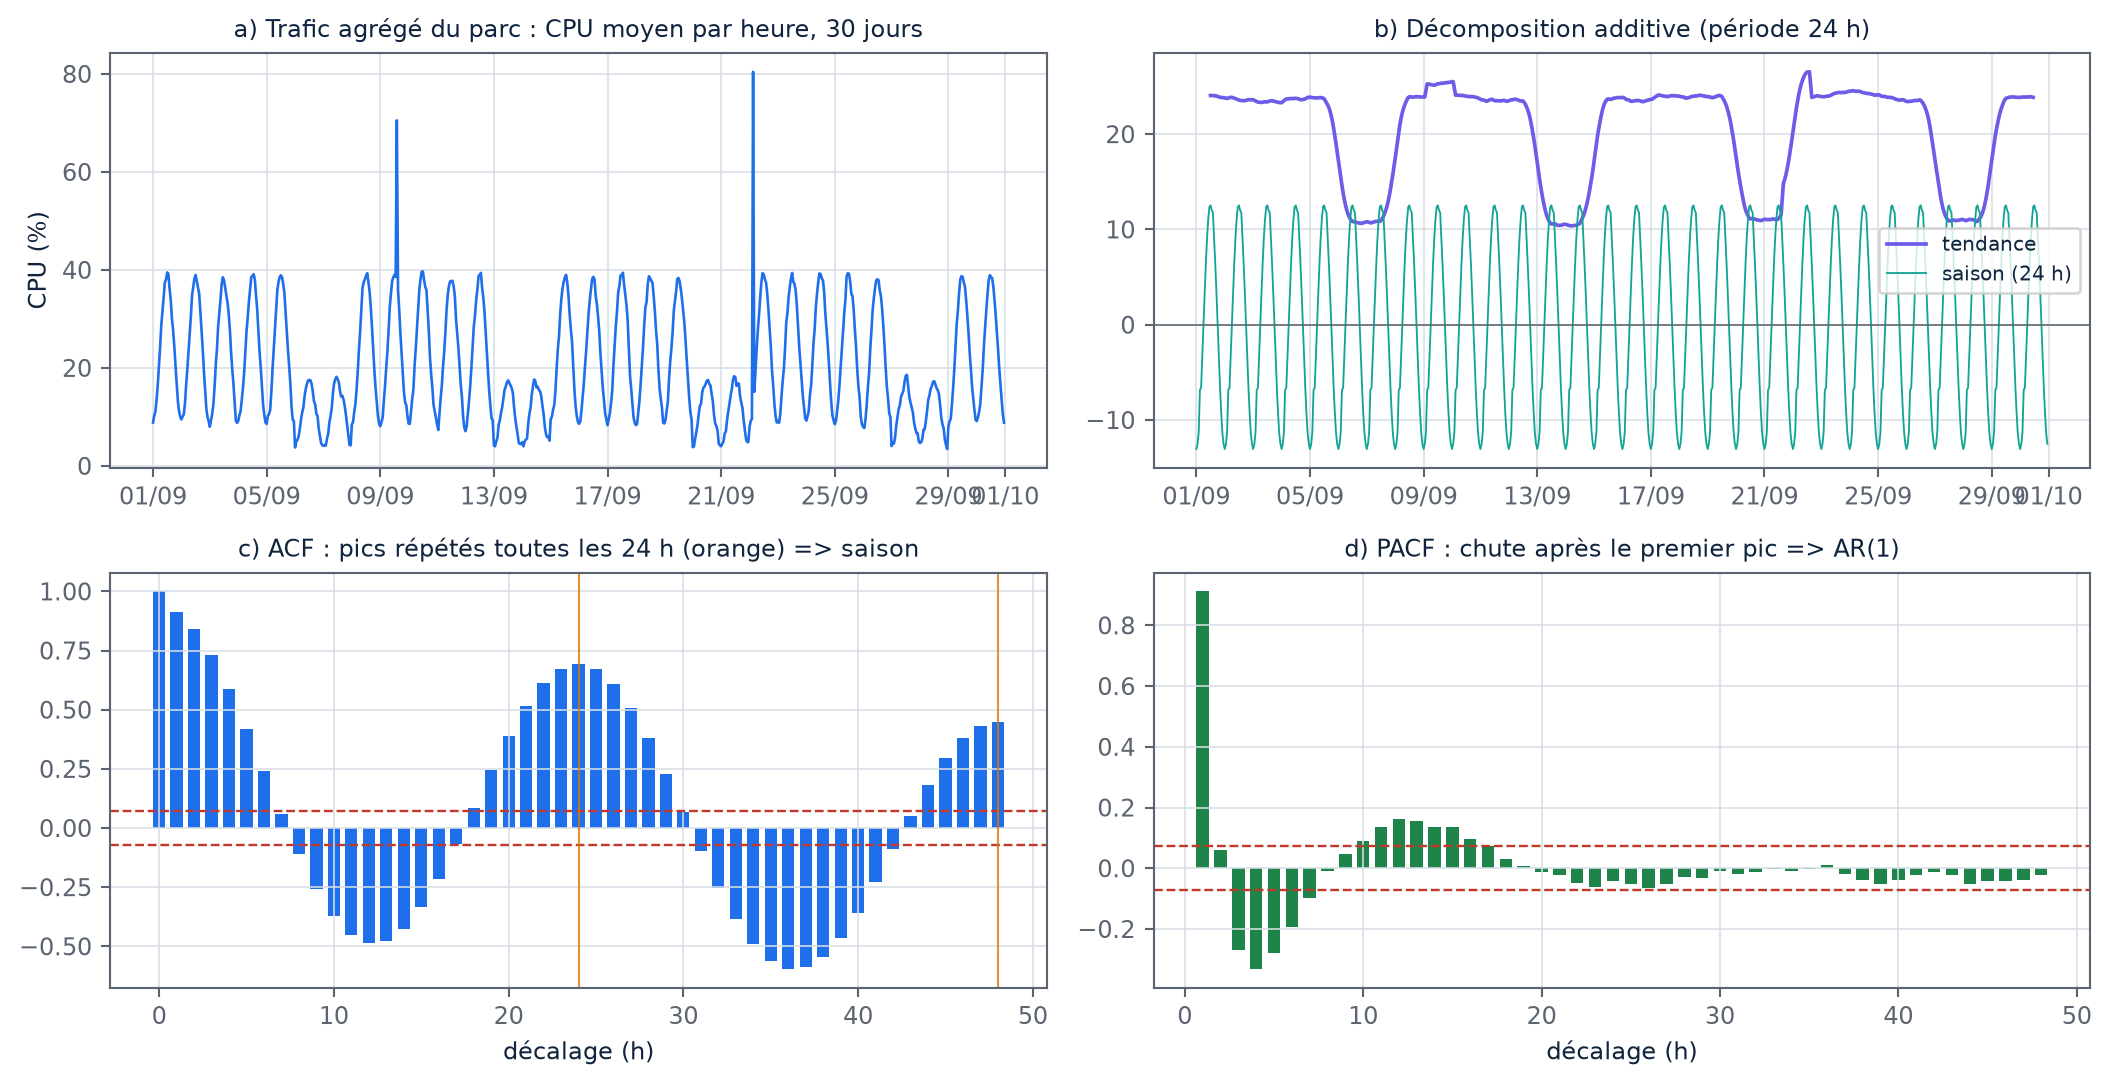
\includegraphics[width=0.82\textwidth]{f25_decomposition_acf.png}
\end{center}
\vspace{-1mm}
\begin{kbox}[Comment lire]
\small
\textbf{ACF} qui décroît lentement = non stationnarité ; pics répétés
toutes les 24 h = \textbf{saison journalière}. \textbf{PACF} qui chute
après le premier retard = \textbf{AR(1)}. Ces graphiques donnent le
premier candidat : $p$ $\approx$ retards PACF, $q$ $\approx$ retards
ACF, saison au lag 24.
\end{kbox}
\end{frame}

\begin{frame}{ARIMA : que signifient p, d, q ?}
\begin{center}\small
\begin{tabular}{@{}p{1.4cm}p{5.6cm}p{4.6cm}@{}}
\toprule
\textbf{Param.} & \textbf{Signification} & \textbf{Comment le choisir}\\
\midrule
$p$ & \textbf{AR} : régression sur les $p$ valeurs passées & retards
significatifs de la \textbf{PACF}\\
\addlinespace[1pt]
$d$ & \textbf{différenciation} : nb de fois où l'on soustrait la valeur
précédente pour stabiliser & test \textbf{ADF} (le minimum qui stationnarise)\\
\addlinespace[1pt]
$q$ & \textbf{MA} : régression sur les $q$ erreurs passées & retards
significatifs de l'\textbf{ACF}\\
\bottomrule
\end{tabular}
\end{center}
\vspace{1mm}
\begin{ebox}[Version saisonnière SARIMA$(p,d,q)(P,D,Q)_s$]
Mêmes trois nombres, appliqués au \textbf{retard saisonnier} $s$ : ici
$s = 24$ (agrégat horaire). À 5 min on aurait $s = 288$, à 15 min
$s = 96$ --- lourds : d'où notre agrégation à l'heure.
\end{ebox}
\vspace{1mm}
\begin{center}\small
Notation du dossier : SARIMA$(p,d,q)\times(P,D,Q)_{24}$ --- on choisit la
grille par \textbf{AIC} (qualité de l'ajustement pénalisée par la
complexité).
\end{center}
\end{frame}

\begin{frame}{Le SARIMA du dossier, réellement ajusté}
\begin{columns}[t]
\begin{column}{0.52\textwidth}
\begin{block}{Protocole (graine 5534, 2 threads)}
\begin{itemize}
\item entraînement : 24 premiers jours = \textbf{576 points} ;
\item grille $(p,0,q) \times (1,0,1)_{24}$, harmoniques hebdomadaires
en exogènes (la semaine se connaît d'avance, comme l'heure) ;
\item sélection par \textbf{AIC}, prévision des 6 jours suivants.
\end{itemize}
\end{block}
\begin{solbox}[Résultats mesurés]
Meilleur ordre : SARIMA$(2,0,1)\times(1,0,1)_{24}$
(AIC 3\,121,5). \textbf{MAE test = 3,01 pts CPU} contre 5,06
(persistance 24 h) et 5,23 (semaine précédente) : \textbf{$-40{,}5$ \%}
d'erreur.
\end{solbox}
\end{column}
\begin{column}{0.44\textwidth}
\begin{wbox}[Résidus : le modèle n'est pas parfait]
Ljung-Box sur les résidus (lag 24) : $p < 0{,}001$ --- il reste de
l'autocorrélation. Traduction : le SARIMA capte tendance + cycles, mais
les \textbf{incidents} (pics) échappent encore au modèle.
\footnotesize Une phrase à retenir : \emph{le test de Ljung-Box vérifie
que les résidus ne contiennent plus de structure temporelle exploitable.}
\end{wbox}
\end{column}
\end{columns}
\end{frame}

\begin{frame}{Quiz 1 --- séries temporelles (5 min)}
\begin{qbox}[3 questions]
\begin{enumerate}
\item Une série dont l'ACF décroît très lentement est probablement :\\
(a) stationnaire \quad (b) non stationnaire --- il faut différencier \quad
(c) saisonnière seulement
\item À 5 min de granularité, la saison journalière vaut :\\
(a) $s = 24$ \quad (b) $s = 96$ \quad (c) $s = 288$
\item Sur notre série, l'ADF donne $p = 0{,}075$ sur la série brute. Que
fait-on ?\\
(a) on accepte la stationnarité \quad (b) on différencie et on reteste
\quad (c) on augmente $q$
\end{enumerate}
\end{qbox}
\vspace{1mm}
\begin{solbox}[Réponses]
\textbf{1 : b} \quad \textbf{2 : c} (288 pas de 5 min par jour ; 96 à
15 min ; 24 à l'heure) \quad \textbf{3 : b} --- $p > 0{,}05$ : on ne
rejette pas H0, on différencie ($d$ ou $D$) puis on reteste.
\end{solbox}
\end{frame}
